
 \newcommand{\markovPairwise}{
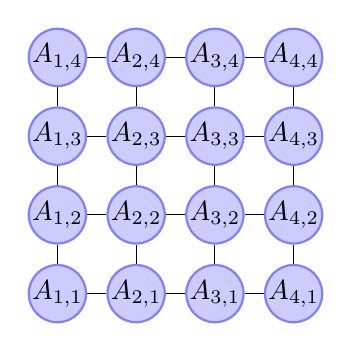
\begin{tikzpicture}
[mynode/.style={circle,draw=blue!50,fill=blue!20,thick, inner sep=0pt,minimum size=5mm}]

\node (n11) at ( 0,0) [mynode] {$A_{1,1}$};
\node (n12) at ( 0,1) [mynode] {$A_{1,2}$};
\node (n13) at ( 0,2) [mynode] {$A_{1,3}$};
\node (n14) at ( 0,3) [mynode] {$A_{1,4}$};

\node (n21) at ( 1,0) [mynode] {$A_{2,1}$};
\node (n22) at ( 1,1) [mynode] {$A_{2,2}$};
\node (n23) at ( 1,2) [mynode] {$A_{2,3}$};
\node (n24) at ( 1,3) [mynode] {$A_{2,4}$};

\node (n31) at ( 2,0) [mynode] {$A_{3,1}$};
\node (n32) at ( 2,1) [mynode] {$A_{3,2}$};
\node (n33) at ( 2,2) [mynode] {$A_{3,3}$};
\node (n34) at ( 2,3) [mynode] {$A_{3,4}$};

\node (n41) at ( 3,0) [mynode] {$A_{4,1}$};
\node (n42) at ( 3,1) [mynode] {$A_{4,2}$};
\node (n43) at ( 3,2) [mynode] {$A_{4,3}$};
\node (n44) at ( 3,3) [mynode] {$A_{4,4}$};

\foreach \from/\to in {n11/n21,n21/n31,n31/n41, n12/n22,n22/n32,n32/n42, n13/n23,n23/n33,n33/n43, n14/n24,n24/n34,n34/n44} 
	\draw (\from) -- (\to);

\foreach \from/\to in {n11/n12,n21/n22,n31/n32,n41/n42, n12/n13,n22/n23,n32/n33,n42/n43, n13/n14,n23/n24,n33/n34,n43/n44} 
	\draw (\from) -- (\to);

\end{tikzpicture}
}


\newcommand{\markovABCD}{
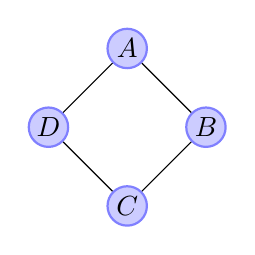
\begin{tikzpicture}
[mynode/.style={circle,draw=blue!50,fill=blue!20,thick, inner sep=0pt,minimum size=5mm}]
\node (A) at ( 0,1) [mynode] {$A$};
\node (B) at ( 1,0) [mynode] {$B$};
\node (C) at ( 0,-1) [mynode] {$C$};
\node (D) at ( -1,0) [mynode] {$D$};
\draw (A) -- (B);
\draw (B) -- (C);
\draw (C) -- (D);
\draw (D) -- (A);

\end{tikzpicture}
 } 
 
\newcommand{\bayesianABCD}{
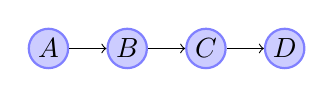
\begin{tikzpicture}
[mynode/.style={circle,draw=blue!50,fill=blue!20,thick, inner sep=0pt,minimum size=5mm}]
\node (A) at ( 0,0) [mynode] {$A$};
\node (B) at ( 1,0) [mynode] {$B$};
\node (C) at ( 2,0) [mynode] {$C$};
\node (D) at ( 3,0) [mynode] {$D$};

\foreach \from/\to in {A/B, B/C, C/D}
	\draw [->]  (\from) -- (\to);

\end{tikzpicture}
 } 
 
 
\newcommand{\bayesianStudentExample}{
\begin{tikzpicture}
\tikzstyle{mynode} = [ellipse,draw=blue!50,fill=blue!20,thick, inner sep=0pt,minimum width=15mm, minimum height=5mm, line width=1.25pt]
\node (D) at (-1,2) [mynode] {$Difficulty$};
\node (I) at ( 1.5,2) [mynode] {$Intelligence$};
\node (G) at (0,1) [mynode] {$Grade$};
\node (S) at (2.5,1) [mynode] {$SAT$};
\node (L) at (0,0) [mynode] {$Letter$};

\foreach \from/\to in {D/G, I/G, G/L, I/S}
	\draw [line width=1.25pt, ->]  (\from) -- (\to);

\end{tikzpicture}
 } 

